\blinddocument

\section{Test}

\begin{minted}[mathescape, linenos]{python}

    # Note: $\pi=\lim_{n\to\infty}\frac{P_n}{d}$
    title = "Hello World"
    
    sum = 0
    for i in range(10):
     sum += i
\end{minted}

\begin{figure}
    \centering
    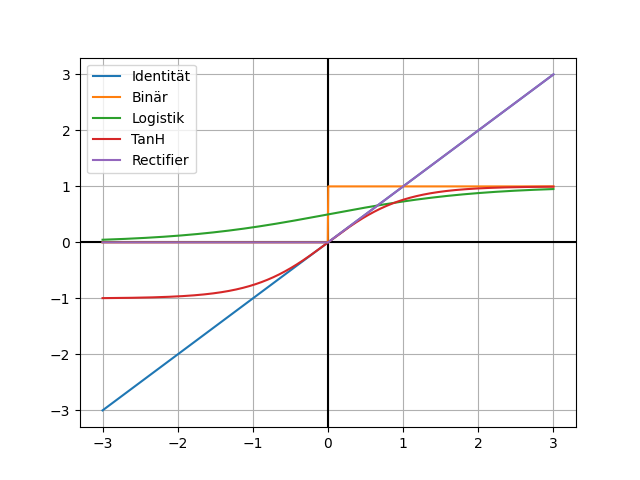
\includegraphics[width=0.8\textwidth]{img/test.png}
    \caption{Einige typische Aktivierungsfunktionen}
    \label{fig:actfn}
\end{figure}


\begin{table}[h!]
    \begin{center}
      \caption{More rows.}
      \label{tab:table1}
      \begin{tabular}{l|S|r}
        \textbf{Value 1} & \textbf{Value 2} & \textbf{Value 3}\\
        $\alpha$ & $\beta$ & $\gamma$ \\
        \hline
        1 & 1110.1 & a\\
        2 & 10.1 & b\\
        3 & 23.113231 & c\\
        4 & 25.113231 & d\\ % <-- added row here
      \end{tabular}
    \end{center}
  \end{table}

after minted
this works 
Objekte
\cite{juliani2018unity}

\blinddocument